\section{Latch D \label{sec:s2}}

\begin{center}
	\begin{minipage}{12cm}
		\begin{tcolorbox}[title=Actividad 2]
			Considerar la tabla ``\textit{ONE – HOT} modificada'':\enter
			
				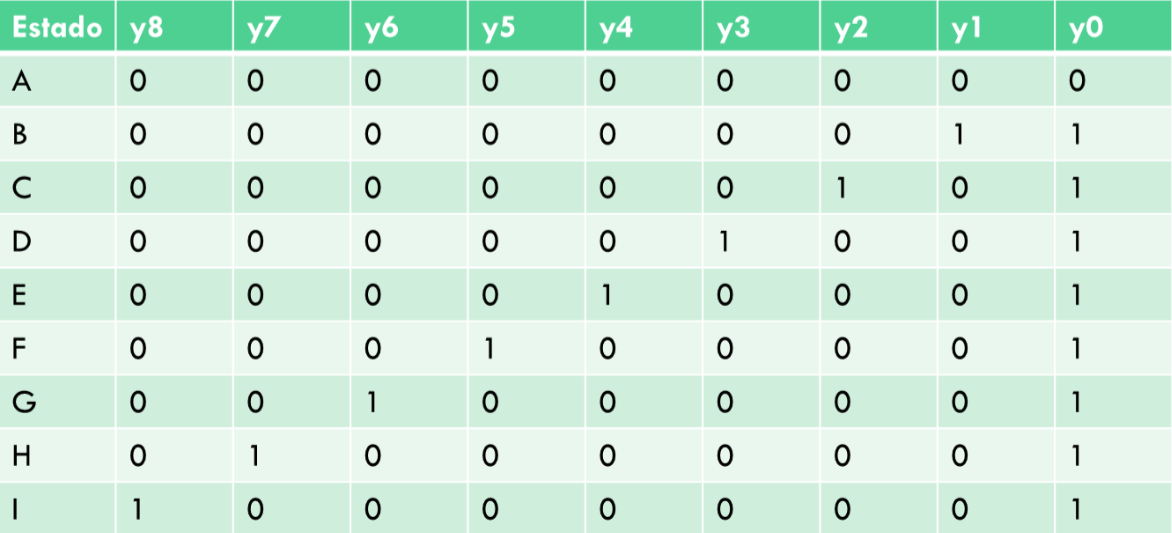
\includegraphics[scale=0.3,center]{OneHotModified.png}
			Diseñar utilizando las ecuaciones de los flip-flops de la tabla modificada. Observar el resultado en el visor RTL. Compilar y simular.
		\end{tcolorbox}	
	\end{minipage}
\end{center}

La visualización RTL del latch D, implementado con la directiva \textit{keep}, se muestra en la \autoref{fig:Latch_D_Keep_RTL} y sin esta directiva en la \autoref{fig:Latch_D_NoKeep_RTL}. Los módulos se diferencian en que el circuito con \textit{keep} conserva más compuertas lógicas que el que no usa la directiva, además de mantener intactas a las señales internas.

La visualización con el \textit{Technology Map Viewer} del latch D, implementado con la directiva \textit{keep}, se muestra en la \autoref{fig:Latch_D_Keep_TMV} y sin esta directiva en la \autoref{fig:Latch_D_NoKeep_TMV}. Los módulos se diferencian en que el circuito con \textit{keep} implementa una celda lógica por cada señal interna declarada en el código, mientras que el circuito sin \textit{keep} emplea una sola celda lógica para todo el circuito.

Las simulaciones sin retardos se visualizan en la \autoref{fig:Latch_D_Keep_Wave} para el latch con directiva \textit{keep} y en la \autoref{fig:Latch_D_NoKeep_Wave} para el latch sin directiva. Ambos circuitos funcionan de la misma manera, de tal forma que:

\begin{itemize}
	\item \textbf{Si D = 0}: La salida adquiere un valor bajo.
	\item \textbf{Si D = 1}: La salida adquiere un valor alto.
\end{itemize}

Nótese que los cambios en la salida ocurren unicamente cuando CLK cambia a un nivel lógico alto.

Las simulaciones con retardos (modo lento a 85°C) se visualizan en la \autoref{fig:Latch_D_Keep_Wave85} para el latch con directiva \textit{keep} y en la \autoref{fig:Latch_D_NoKeep_Wave85} para el latch sin directiva. Se observa que, debido a que se simuló en el peor de los escenarios, la señal de salida Q, tarda en actualizar su valor en ambas simulaciones, no obstante, para el caso del circuito con \textit{keep}, el retardo es ligeramente mayor en comparación con el circuito sin \textit{keep}.

En los Anexos se localiza la descripción del latch RS. Además de declarar a las entradas y salidas, se describieron a NAND1, NAND2, NAND3 y NAND4 como señales internas y por medio de la descripción de flujo de datos de bajo nivel, se asignaron los valores de estas señales y de la salida Q. Cabe resaltar que la diferencia entre los circuitos simulados en este apartado, es la directiva \textit{synthesis keep}, en la declaración de las señales internas.

\begin{figure}[ht]
	\centering
	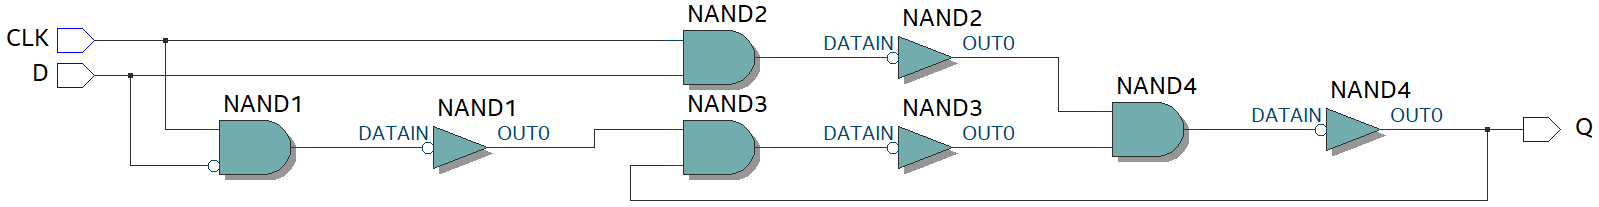
\includegraphics[scale=0.39]{Latch_D_Keep_RTL.png}
	\caption{Diagrama RTL del latch D, descrito con la directiva \textit{keep}. \label{fig:Latch_D_Keep_RTL}}
\end{figure}

\begin{figure}[ht]
	\centering
	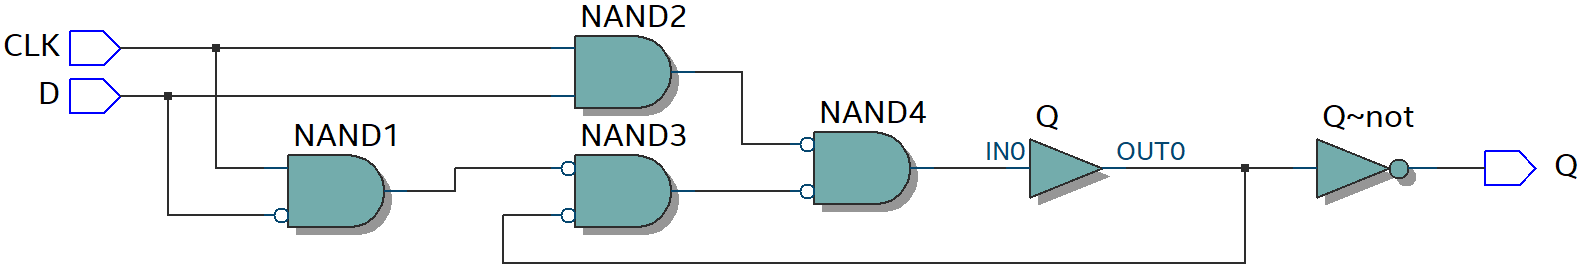
\includegraphics[scale=0.39]{Latch_D_NoKeep_RTL.png}
	\caption{Diagrama RTL del latch D, descrito sin la directiva \textit{keep}. \label{fig:Latch_D_NoKeep_RTL}}
\end{figure}

\begin{figure}[ht]
	\centering
	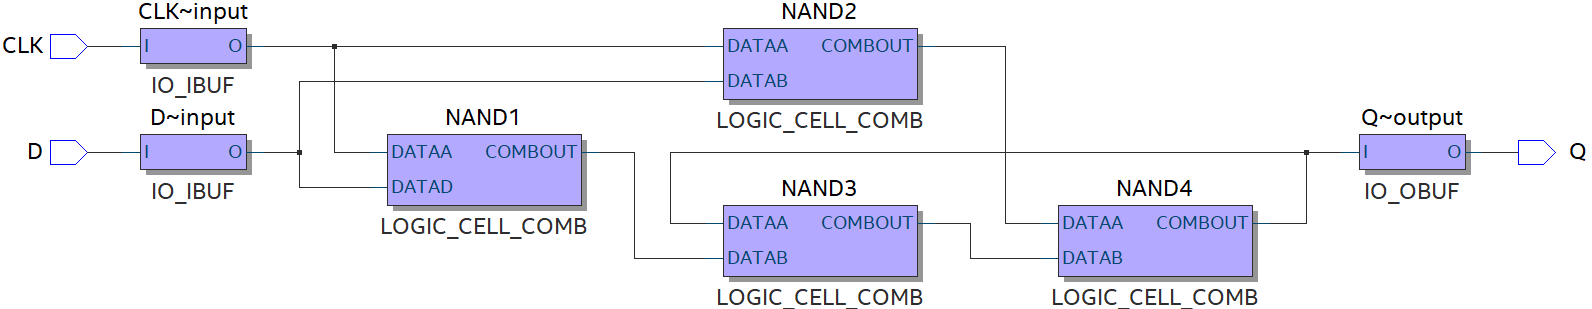
\includegraphics[scale=0.39]{Latch_D_Keep_TMV.png}
	\caption{Latch D (descrito sin la directiva \textit{keep}) visto desde el \textit{Technology Map Viewer}. \label{fig:Latch_D_Keep_TMV}}
\end{figure}

\begin{figure}[ht]
	\centering
	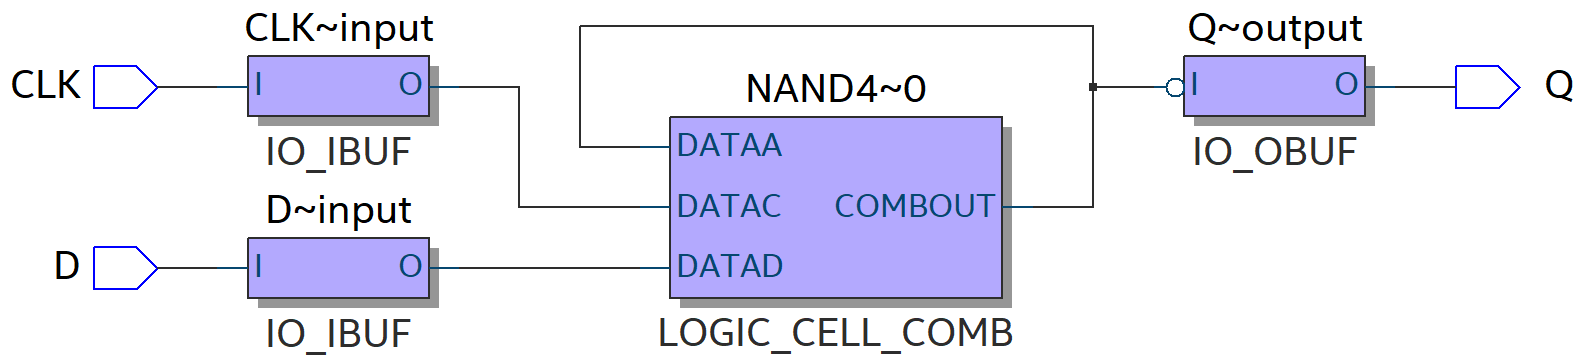
\includegraphics[scale=0.39]{Latch_D_NoKeep_TMV.png}
	\caption{Latch D (descrito sin la directiva \textit{keep}) visto desde el \textit{Technology Map Viewer}. \label{fig:Latch_D_NoKeep_TMV}}
\end{figure}

\begin{figure}[ht]
	\centering
	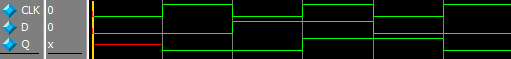
\includegraphics[scale=1.2]{Latch_D_Keep_Wave.png}
	\caption{Simulación sin retardos del latch D (descrito con la directiva \textit{keep}) en el visor de formas de onda de ModelSim. \label{fig:Latch_D_Keep_Wave}}
\end{figure}

\begin{figure}[ht]
	\centering
	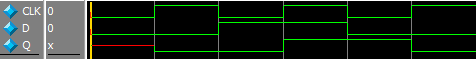
\includegraphics[scale=1.3]{Latch_D_NoKeep_Wave.png}
	\caption{Simulación sin retardos del latch D (descrito sin la directiva \textit{keep}) en el visor de formas de onda de ModelSim. \label{fig:Latch_D_NoKeep_Wave}}
\end{figure}

\begin{figure}[ht]
	\centering
	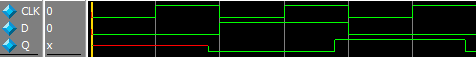
\includegraphics[scale=1.3]{Latch_D_Keep_Wave85.png}
	\caption{Simulación con retardos del latch D (descrito con la directiva \textit{keep}) en el visor de formas de onda de ModelSim. \label{fig:Latch_D_Keep_Wave85}}
\end{figure}

\begin{figure}[ht]
	\centering
	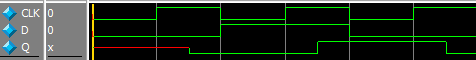
\includegraphics[scale=1.3]{Latch_D_NoKeep_Wave85.png}
	\caption{Simulación sin retardos del latch D (descrito sin la directiva \textit{keep}) en el visor de formas de onda de ModelSim. \label{fig:Latch_D_NoKeep_Wave85}}
\end{figure}